
\documentclass[english]{paper}
\usepackage[T1]{fontenc}
\usepackage[latin9]{inputenc}
\usepackage{geometry}
\geometry{verbose,tmargin=3cm,bmargin=3cm,lmargin=2cm,rmargin=2cm}
\usepackage{fancyhdr}
\pagestyle{fancy}
\usepackage{color}
\usepackage{babel}
\usepackage{fancybox}
\usepackage{calc}
\usepackage{units}
\usepackage{amsmath}
\usepackage{stackrel}
\usepackage{graphicx}
\usepackage{setspace}
\onehalfspacing
\usepackage[unicode=true]
 {hyperref}

\makeatletter

\providecommand{\tabularnewline}{\\}

\usepackage{lineno}
\linenumbers


\makeatother

\begin{document}

\chead{\textbf{\textcolor{red}{FOR YOUR EYES ONLY! DO NOT SHARE!}}\\
\textbf{\textcolor{red}{Contains instructions for an attack on Monero
users' privacy!}}\\
}
\title{\textcolor{red}{\Large{}FOR YOUR EYES ONLY! DO NOT SHARE!}\\
\textcolor{red}{\Large{}Contains instructions for an attack on Monero
users' privacy!}\\
Research Roadmap for an Overhaul of Monero's Mixin Selection Algorithm}
\author{Rucknium}

\maketitle

2021-09-16


\begin{abstract}
This document discusses the shortcomings of Monero's current mixin
selection algorithm, a specific attack that exploits those shortcomings,
and a plan to overhaul the algorithm so as to eliminate those shortcomings.
I first challenge the widely-believed notion that the the true spend-age
distribution is knowable by explaining a simple way to estimate it.
I then develop the Rucknium Ratio Attack (RRA), a potent attack on
user privacy that could allow tracing of about 35 percent of all transactions
that have been confirmed on the Monero blockchain since the recommendation
of M{\"o}ser et al. (2018) was implemented. Finally, I outline a long-term
solution to the problem in the form of nonparametric estimation of
the true spend-age distribution. I close with a medium-term solution
--- Optimal Static Parametric Estimation of Arbitrary Distributions
(OSPEAD) --- that is probably implementable within a few months.
\end{abstract}
\noindent\doublebox{\begin{minipage}[t]{1\columnwidth - 2\fboxsep - 7.5\fboxrule - 1pt}%
\textbf{NOTE TO VULNERABILITY RESPONSE PROCESS REVIEWERS}: The main
thing I want to result from this submission is an official determination
of what should be redacted from a public version of this document
in order to protect user privacy. I give my own view about information
exclusions in Recommendation III. I wish to submit a CCS funding proposal
that is based on this ``roadmap'', so your views on redactions is
appreciated. The organization and tone of this roadmap will likely
change before release, but the basic elements are all here. The second
thing is to initiate the Monero process for mitigating vulnerabilities,
whatever that may be. The third and final thing is to determine if
this submission qualifies for a vulnerability bug bounty. I have attached
an XMR address for use if a bounty is deemed warranted. I initially
offered jberman 50 percent of any bounty due to his substantial contribution
to the advances contained herein, but he has declined any payment
for this particular submission. I thank jberman and isthmus for their
reviews of drafts of this document; the two of them plus Syksy would
be good auxiliary reviewers for this submission. jberman and isthmus
have been provided copies of this final version of the submission.\\

Developing an attack on user privacy is an inherently dangerous affair,
but I did it for the following reasons. First, the attack formed in
my mind as a natural result of thinking of how to fix the mixin selection
algorithm. Second, the existence of this attack should remove all
doubt about the importance of addressing weaknesses in the current
mixin selection algorithm. Third, knowledge of a specific attack can
help in developing a fix to the mixin selection algorithm, since any
proposed solution's resistance to this specific attack can be measured
precisely.\\
\\
In order to prove first discovery of the Rucknium Ratio Attack if
it were to be independently developed and published publicly by someone
else, I plan to hash this document and, separately, certain individual
sections and embed the hash in the OP\_RETURN of transactions on the
BTC and BCH blockchains within the next week. I believe that doing
so carries no risk, but please let me know if there would be any concerns.\\
\\
Just as I was finishing this submission, I was made aware of \href{https://petsymposium.org/2021/files/papers/issue3/popets-2021-0047.pdf}{Ronge, Egger, Lai, Schr{\"o}der, and Yin (2021), \textquotedblleft Foundations of Ring Sampling,\textquotedblright}
which lays out a formal framework for mixin selection algorithms.
I have not had time to examine the paper closely. However, it is worth
noting that they claim that estimating the real spend-age distribution
is not feasible as a practical matter. I show below that this claim
is false. Importantly, the fact that this claim is made does suggest
that the broader computer science community remains somewhat clueless
about the possibility of estimating the real spend-age distribution,
and therefore its use as ammunition in a potential attack. This suggests
that indefinite nondisclosure of the details of the Rucknium Ratio
Attack and its foundations could be beneficial and advisable.%
\end{minipage}}\\
\\


\section{The mixin selection algorithm is in need of attention by qualified
statisticians}

$\vphantom{}$

Let $f_{S}(x)$ denote the probability density function (PDF) of the
age of the real spend outputs of transactions on the Monero blockchain.\footnote{Strictly speaking, $f_{S}(x)$ and $f_{M}(x)$ are both probability
mass functions (PMFs) since block age is discrete, but for expositional
simplicity I will treat them as PDFs.}

Let $f_{M}(x)$ denote the PDF of the age of the mixins used by the
reference wallet software for Monero.\\

\textbf{My unvarnished view:}\\

The gamma probability density function (PDF) with shape parameter
19.28 and rate 1.61 suggested by M{\"o}ser et al. (2018) was a decent
first draft for approximating $f_{S}(x)$ especially given that the
paper covered a lot of other ground. However, in my view it never
should have been used in production code. Even if it were to have
been used in production code, the estimates should have been updated
regularly, given the changing spend-age dynamics over time.

I am not one for conspiracy theories, but keep in mind that one of
the authors of the paper (Andrew Miller) was on the board of the Zcash
Foundation at the time of its publication and now. Other authors disclose
that their research was financially supported by the U.S. National
Science Foundation and the U.S. Department of Homeland Security. The
authors would have little incentive to develop an unassailable mixin
selection algorithm even if they were capable of doing so.

Speaking of capability of doing so: If the authors had a deep understanding
of statistical methods, they did not show it in this paper. I have
heard of the concept of \textquotedbl code smell\textquotedbl{} in
programming, and here I analogously detected a \textquotedbl statistics
smell\textquotedbl . It was not a good smell. I would be happy to
go into detail, but to summarize there are many lapses in statistical
rigor, especially in the key section on countermeasures. In my experience,
many computer scientists know \textquotedbl just enough to be dangerous\textquotedbl{}
when it comes to statistics, especially when they try to work with
data derived from human behavior. I am not really sure what statistics
training for a typical computer scientist is, but from some observations
it seems to me that it concentrates on probability theory rather than
statistics itself. 

Probability theory deals with problems when you know the underlying
probability characteristics of the object under study; you just need
to calculate the data that will be generated from the known stochastic
processes. Statistics, on the other hand, examines the inverse: The
data that is generated is known, but the underlying stochastic process
that generated the data is not known. Statistical problems are generally
more difficult than probability problems and often require substantial
experience with empirical data to determine the best approach. Fortunately,
as an empirical microeconomist my training in statistics is very extensive
as is my experience with empirical data on economic behavior of individuals.

It is no one's fault that the flawed gamma-derived mixin selection
algorithm was adopted into Monero's production code. It would have
been entirely reasonable to assume that a paper with 11 authors, 3
of whom are professors at top universities, would have produced a
reliable algorithm. But this highlights what appears to be a substantial
shortcoming in how Monero's development has proceeded: Apparently
no qualified statisticians have reviewed the protocol of a privacy
model that is dependent upon its resistance to statistical attack
in order to protect user privacy. Or to put it in a more precise,
more alarming way: No statisticians \textit{whose goal is to protect
the privacy of Monero users} have reviewed the protocol. It is highly
likely that a statistician or two is working for those who wish to
de-anonymize Monero users. Of course, Monero developers and researchers
cannot just conjure up statisticians to work on Monero, so statistical
attack has hitherto been a blind spot in Monero's defenses. However,
as the result of some unknown stochastic process I'm here now to help
shore up the weaknesses in the current algorithm, and I may be able
to recruit other statisticians to help.

It is probably the case that the the original developer of Monero,
whoever they were, did not realize the full implications of developing
a privacy protocol that requires statistical obfuscation to ensure
users' privacy. But if we choose to stay on this road, I see no other
choice than to follow it to its necessary destination: minimum leakage
of statistically meaningful data. This could be painful and get complicated.
The alternatives, I see them, are A) Keep the flawed mixin algorithm
and possibly compromise users' privacy; or B) switch to a completely
different privacy model that does not rely on statistical obfuscation.
For example, Zcash, to my knowledge, does not require statistical
obfuscation except for basic user awareness about timing and amount
attacks when transferring coins from the transparent to the shielded
pool and vice versa.

I do not think that an apparently \textquotedbl good enough\textquotedbl{}
mixin selection algorithm is actually good enough. The current algorithm
does provide some minimum safety for the privacy of even the most-exposed
transactions, but as Monero becomes an even more attractive target
for government surveillance, the statistical attacks on privacy will
become increasingly intense. The field of statistics is vast. Vast,
vast, vast. There are currently over 18,000 statistical packages on
the Comprehensive R Archive Network (CRAN). Over 200 of them deal
specifically with mixture distributions --- which would be a first
step of anyone wanting to undermine the privacy of Monero. And this
is not accounting for statistical techniques that may be developed
in the near future. As far as I can see, the best way to defend against
attacks is define $f_{M}(x)$ in a way that minimizes the leakage
of statistically meaningful data.\\

\noindent\doublebox{\begin{minipage}[t]{1\columnwidth - 2\fboxsep - 7.5\fboxrule - 1pt}%
\begin{description}
\item [{\textbf{Recommendation}}] \textbf{I:} Across all software and protocol
development contexts, interdisciplinary collaboration between computer
scientists, statisticians, and other disciplines is essential to eliminate
blind spots that could compromise user privacy. This is a systemic
problem, of course, and the Monero Project cannot hope to solve it
at a global level. However, the Monero Project can lead by example.
\end{description}
%
\end{minipage}}\\

\noindent\doublebox{\begin{minipage}[t]{1\columnwidth - 2\fboxsep - 7.5\fboxrule - 1pt}%
\begin{description}
\item [{\textbf{Recommendation}}] \textbf{II:} The Monero Project should
actively recruit technical talent from universities and university
orbits in order to identify and eliminate vulnerabilities in its protocol.
I outline a sketch of such a recruitment effort \href{https://www.reddit.com/r/Monero/comments/pkg3d6/the_monero_project_should_actively_recruit/}{here}.
\end{description}
%
\end{minipage}}

\section{The age distribution of real spends is recoverable}

It seems from conversations with Monero community members that is
has been believed that obtaining the distribution of real spends was
not possible now that the mixin selection suggestion from M{\"o}ser et
al. (2018) has been implemented. Under some plausible assumptions,
this belief is not at all true.

(Repeating some definitions) Let:

$f(x)$ be the observed spend-age PDF (includes mixins and real spends).
This is known. Or, more precisely, the empirical version of this is
known.

$f_{S}(x)$ be the PDF of the age of the real spend outputs of transactions
on the Monero blockchain. This is unknown (for now).

$f_{M}(x)$ be the PDF of the age of the mixins used by the reference
wallet software for Monero. This is probably known; see below.

$\alpha$ the proportion of ring members that are mixins. This is
known to be $\nicefrac{10}{11}$.

The only important assumption that is needed for the following argument
is that $f_{M}(x)$ is known. I will return to this issue shortly.
For now, assume that $f_{M}(x)$ is known.

These expressions are related in the following way:

\begin{equation}
f(x)=(1-\alpha)\cdot f_{S}(x)+\alpha\cdot f_{M}(x)\label{eq:f(x)}
\end{equation}

Everything in that expression is approximately known, except for $f_{S}(x)$.
Therefore, $f_{S}(x)$ can be calculated by simple arithmetic, basically.
Rearranging (\ref{eq:f(x)}) yields

\begin{equation}
f_{S}(x)=\frac{1}{1-\alpha}\left(f(x)-\alpha\cdot f_{M}(x)\right)\label{eq:f_S(x)}
\end{equation}

Once in hand, $f_{s}(x)$ can likely serve as ammunition for any number
of potent attack weapons. After a bit of thinking, I have developed
one such weapon: the Rucknium Ratio Attack (RRA). The RRA is explained
in the next section, but first let me return to the issue of knowing
$f_{M}(x)$.

Most likely, $f_{M}(x)$ is known since it is written into the code
of the reference wallet. If a substantial proportion of transactions
on the blockchain are created by a wallet that does not use the reference
wallet's mixin selection algorithm, then we only know $f_{M}(x)$
\textquotedbl with error\textquotedbl . The only known wallet that
does not use the reference wallet's mixin selection algorithm is monero-lws/mymonero.com
. The mymonero wallet does not suffer from the integer truncation
bug that has recently been discovered in the reference wallet. The
proportion of transactions on the Monero blockchain that mymonero
has produced is unknown. However, if it is substantial then it might
be estimated via estimation of a mixture distribution.

Isthmus believes that there is a wallet out there that uses a uniform
distribution as well as an ``exchange wallet bug''. Very recently
there have been some discoveries in the course of analyzing the July--August
2021 transaction volume anomaly that could help identify rogue wallets
and their share of total transaction volume. See also jberman's work
\href{https://github.com/monero-project/research-lab/issues/86\#issuecomment-915806414}{here}.
In any case, a Maximum Likelihood Estimation (or similar estimation
technique) of $f_{S}(x)$ and $f_{M}(x)$ could proceed as follows.
Define a decomposition of $f_{M}(x)$ as $f_{M}(x)=\alpha_{1}\cdot f_{M,1}(x)+\alpha_{2}\cdot f_{M,2}(x)+\cdots+\alpha_{N}\cdot f_{M,N}(x)$
where each $f_{M,i}(x)$ is known but the $\alpha_{i}$weights are
unknown. Define $\alpha=\sideset{}{_{i=1}^{N}}\sum\alpha_{i}$. Then
the following mo del could be estimated:

\[
f(x)=(1-\alpha)\cdot f_{S}(x)+\stackrel[i=1]{N}{\sum}\alpha_{i}\cdot f_{M,i}(x)
\]

$f_{s}(x)$would then be a nonparametric ``residual''.

\section{The Rucknium Ratio Attack (RRA)}

\subsection{Definition}

The Rucknium Ratio Attack (RRA) is intuitive and requires the application
of no sophisticated statistical techniques, although as a formal matter
it may amount to a maximum likelihood estimator of some sort. It is
so simple that laypeople --- say, for instance, members of a jury
in a criminal case --- may be able to grasp it intuitively.

As I note later, I have not dotted all i's nor crossed all t's on
the attack since my time is better spent developing defenses to this
attack and any related attacks, but the core of the attack likely
has no fundamental flaws.

The sketch of the attack requires just two steps:
\begin{enumerate}
\item Estimate $f_{S}(x)$ and $f_{M}(x)$ through the procedure outlined
in Section 2 or a similar procedure.
\item Choose any ring of ``interest'' to analyze. The most likely real
spend is then the ring member that comes from the block for which
the following ratio is highest:
\end{enumerate}
\begin{equation}
\dfrac{f_{S}(x)}{f_{M}(x)}\label{eq:Rucknium_Ratio}
\end{equation}

I call (\ref{eq:Rucknium_Ratio}) the Rucknium Ratio. The attack operationalizes
the intuitive idea that the ring member that is most likely to be
the real spend is the ring member that comes from the block where
the real spend distribution is thickest relative to the mixin selection
algorithm's distribution.

A formal definition of the Rucknium Ratio Attack follows.

Let $\boldsymbol{R}=\left\{ r_{1},r_{2},...,r_{11}\right\} $ be the
set of ring members. Without loss of generality, let the real spend
be $r_{11}$.

Let $\boldsymbol{B}=\left\{ b_{1},b_{2},...,b_{11}\right\} $ be the
block heights of the blocks that each ring member $r$ was originally
confirmed in.

Let $RRA$, the Rucknium Ratio Attack, be a function that maps the
set of ring members onto itself, i.e.

$RRA:\boldsymbol{R}\rightarrow\boldsymbol{R}$

As we will see in a moment, $RRA$ can be a many-to-many function
or a many-to-one function.

Finally, define $RRA$ as follows:

\begin{equation}
RRA(\boldsymbol{R})\equiv\underset{r_{i}\in\boldsymbol{R},b_{i}\in\boldsymbol{B}}{\mathrm{argmax}}\left\{ \dfrac{f_{S}(b_{i})}{f_{M}(b_{i})}\right\} \label{eq:RRA_formal}
\end{equation}

where each element $b_{i}$ of $\boldsymbol{B}$ corresponds to its
counterpart element $r_{i}$ in $\boldsymbol{R}$.

$RRA$ will not necessarily produce a singleton since it is possible
for multiple ring members to come from the same block. It is also
possible that the Rucknium Ratio $\frac{f_{S}(x)}{f_{M}(x)}$ is identical
for distinct elements of $\boldsymbol{B}$. In that case, application
of the $RRA$ function to a particular $\boldsymbol{R}$ would produce
a set with multiple elements.

The probability that the RRA correctly and uniquely guesses the true
spend for any given $\boldsymbol{R}$ is then:

\begin{equation}
Pr\left(\text{{guess\:real\:spend\:correctly}}|\boldsymbol{R}\right)=Pr\left(RRA(\boldsymbol{R})=\left\{ r_{11}\right\} |\boldsymbol{R}\right)\label{eq:guess_real_spend}
\end{equation}


\subsection{Simulations with real data demonstrate the potency of the RRA}

As stated in Section 2, there are some very surmountable challenges
in calculating $f_{M}(x)$. Assume for the moment that $f_{M}(x)$
is calculated. Specifically, let $f_{M}(x)$ be the distribution generated
by the official wallet implementation. Then let $f$(x) be the observed
distribution of ring member ages. jberman produced \href{https://github.com/monero-project/monero/files/6968268/output_age_data.zip}{this exact data}
for \href{https://github.com/monero-project/monero/pull/7821}{his analysis of his pull request \#7821}.
The \texttt{Observed} and \texttt{Current decoy selection algo} columns
represent frequency data that can be converted into approximations
of $f(x)$ and $f_{M}(x)$, respectively, by normalizations. Then
$f_{S}(x)$ can be computed by application of equation (\ref{eq:f_S(x)}).
Note that due to the long thin tails of the distributions and the
noisy nature of the empirical data and jberman's simulated data, it
can be the case that the calculated value of $f_{S}(x)$ can be negative
for some values of $x$, which violates an axiom of probability theory.
In those cases, the negative value of $f_{S}(x)$ was replaced by
$f_{M}(x)$, since that would be the most conservative approach.

Figure 1 plots the Rucknium Ratio for the most recent 10,000 blocks.
The Rucknium Ratio is unacceptably high for the first 10 blocks or
so. Also of note are the apparent cycles, possibly on a 24-hour basis,
displayed in the plot.

\begin{figure}
\caption{}

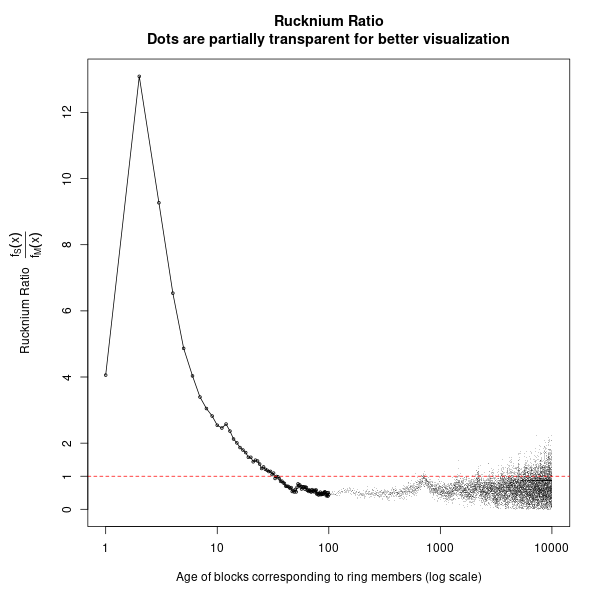
\includegraphics[scale=0.75]{images/Rucknium-Ratio}
\end{figure}

A Monte Carlo simulation can proceed as follows. Construct 10 million
rings. This can be done by drawing 110 million pseudorandom observations
from the estimated $f_{M}(x)$ and 10 million pseudorandom observations
from $f_{S}(x)$. Form up the rings appropriately and apply the RRA
to each ring. The simulated probability of success of the RRA as in
(\ref{eq:guess_real_spend}) for an arbitrary ring is then obtained.
R code for carrying out this simulation is in Appendix A: RRA simulation
code and attached to this document as a separate file.

\textbf{With this simple attack, the simulated probability of successfully
guessing the real spend is about 35.4 percent.} If the existing $f_{M}(x)$
was doing its job perfectly, this figure would be only $\nicefrac{1}{11}\approx9.1$
percent. Note that the simulation is conducted with the assumption
that the $f_{M}(s)$ of the empirical data is known. Note also that
the data that this simulation is based on is from a blockchain ``epoch''
before jberman's fix in PR \#7821 was applied.

\subsection{Increasing the ring size mitigates the vulnerability only weakly}

Not only is the current mixin selection algorithm vulnerable to the
RRA, but the Monero Project's plans to increase ring size only slightly
reducing the attack potency. Only focusing on increasing the ring
size is analogous to producing a lot of camouflage but yet not putting
it in the right places to cover the vulnerable entity. Overhauling
the mixin selection algorithm should therefore be made a high priority.
Via simulations, the effect of increasing the ring size on the potency
of the RRA can be estimated. 

We can simply repeat the same simulation described in Section 3.2,
but for every ring size 2 -- 256 instead of just a single ring size
of 11. To keep the computational burden reasonable, the number of
constructed rings will be reduced to 1 million.

Figure 2 displays the simulated probability of success of the RRA
as in (\ref{eq:guess_real_spend}) as a function of ring size. The
graph roughly traces out a shape of exponential decay. Even with a
ring size of 256, the simulated probability of a correct guess of
the real spend when the RRA is applied is about 8.5 percent. This
may be considered an ``acceptable'' rate of guessibility, but it
is a far cry from $\nicefrac{1}{256}\approx0.39$ percent, which is
what it would be if $f_{M}(x)$ perfectly matched $f_{S}(x)$.

At first glance, the slow fall-off in the potency of the RRA as ring
size increases may seem incredible, but consider the following back-of-the-envelop
illustration. About 13.8 percent of the mass of $f_{S}(x)$ is in
the most recent 10 blocks alone. Only about 2.7 percent of the mass
of $f_{M}(x)$ is in the most recent 10 blocks. Looking more closely,
about 5.52 percent of the mass of $f_{S}(x)$ is in the most recent
3 blocks; for $f_{m}(x)$ the corresponding figure is 0.576 percent.
Therefore, the probability of zero mixins of 255 being drawn from
the most recent 3 blocks is:

$(1-0.00576)^{255}=0.229$

And since the real spend and the mixins are independent, the following
is the probability that no mixins were drawn from the most recent
3 blocks, but the real spend does come from one of the first three
blocks:

$0.229\cdot0.0552=0.01265$

So just the first 3 blocks contribute, in a sense, 1.265 percentage
points of the 8.5 percentage points of total guessibility with ring
size 256.

\begin{figure}
\caption{}

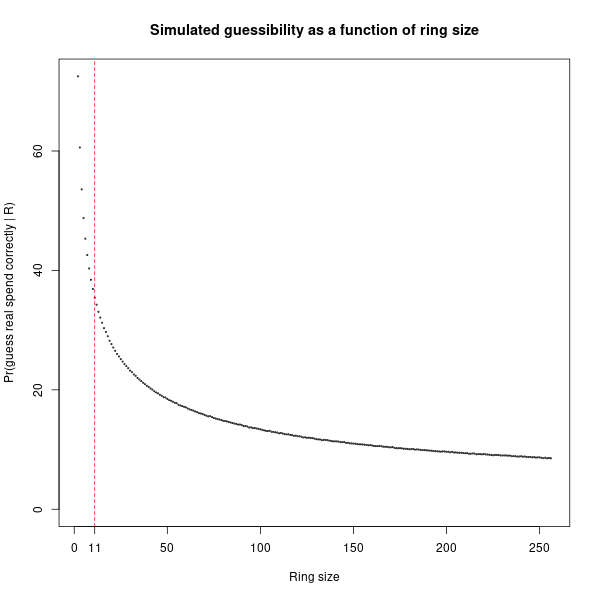
\includegraphics[scale=0.75]{images/Guessibility-by-ring-size}
\end{figure}


\subsection{Enhancements and extensions of the RRA}

Isthmus believes that certain enhancements of the RRA are possible.
These take two forms:
\begin{enumerate}
\item If particular nonstandard forms of $f_{M}(x)$ can be identified,
then transaction ``chains'' that can clearly be identified as using
the nonstandard wallets would be particularly vulnerable to analysis.
\item The RRA could be combined with attack outlined in \href{https://www.overleaf.com/read/ccbmjkrhmrxk}{MRL-0011}
so as to:
\begin{enumerate}
\item inform the edge weights with newfound knowledge of $f_{S}(x)$; and
\item use ``matches'' from the RRA to inform the initial guesses for the
MRL-0011 attack.
\end{enumerate}
\end{enumerate}
Isthmus believes that combining the RRA with MRL-0011 could be ``potentially
catastrophic''.\\

\noindent\doublebox{\begin{minipage}[t]{1\columnwidth - 2\fboxsep - 7.5\fboxrule - 1pt}%
\begin{description}
\item [{\textbf{Recommendation}}] \textbf{III}: Information about the Rucknium
Ratio Attack should never be released publicly, even after a ``patch''.
Due to the distributed and immutable nature of Monero's blockchain,
all transactions since 2018 would remain vulnerable to the attack
regardless of any actions taken by the Monero Project or users now
or in the future. Knowledge about the attack should only be revealed
to select trusted individuals on a need-to-know basis. I would go
further and say that all information in Section 2, especially equations
(\ref{eq:f(x)}) and (\ref{eq:f_S(x)}), should also not be made public.
This is a bit tricky since an improved mixin selection algorithm would
be based on Section 2. However, revealing the methods in Section (2)
are not necessary to implement a ``patch'' in the code, at least
for OSPEAD (explained later), so the only tricky part is to have users
accept ``just trust us'' as a response to any queries about how
we are estimating $f_{S}(x)$. \\
Concealing information about how to develop an attack would not prevent
the Monero Project from issuing an advisory to users that certain
past behavior, such as spending outputs before $z$ blocks had been
confirmed, could expose them to risk --- and therefore they should
take whatever action necessary to protect themselves from exposure
in the event that an adversary were to develop the RRA or similar
attack. Any such public advisory regarding a specified $z$ number
of block confirmations could be based on an analysis of the Rucknium
Ratio, yet any hint of the existence of the Rucknium Ratio and its
significance can be excluded from such an advisory.
\end{description}
%
\end{minipage}}

\section{Mitigation of the vulnerability}

The scope for mitigation of the vulnerability without changes to the
mixin selection algorithm is probably limited. Transactions already
confirmed on the blockchain obviously cannot be altered and would
remain vulnerable to the RRA forever. There may be some user-level
actions available to mitigate the vulnerability for individual users,
but a general recommendation to all Monero users could be counterproductive.
If, for instance, a general recommendation was issued to wait until
$z$ blocks had been confirmed before spending an output in order
to avoid the high Rucknium Ratio for young outputs, then what would
likely happen would be a pile-up of the density of $f_{S}(x)$ at
$x=z$. This would result in arise of the Rucknium Ratio at point
$z$, which would create the same vulnerability all over again, but
just at a different $x$ value. The Monero Project could hardly issue
a recommendation to users of ``Please coordinate among yourselves
so as to spend your outputs at a roughly random uniform distribution
between $z_{a}$ and $z_{b}$ blocks''.

jberman's recent fix to the bug in the wallet that prevented applying
the gamma distribution from the chaintip (\href{https://github.com/monero-project/monero/pull/7821}{PR \#7821})
does alleviate the problem somewhat by reducing the Rucknium Ratio
for the most recent blocks. However, even with the fix, the problem
remains

The only way forward, as far as I see it, is to launch a research
project whose goal is to fix the mixin algorithm itself. \\

\noindent\doublebox{\begin{minipage}[t]{1\columnwidth - 2\fboxsep - 7.5\fboxrule - 1pt}%
\begin{description}
\item [{\textbf{Recommendation}}] \textbf{IV}: The Monero Project should
launch a research project to develop a nonparametric estimate of $f_{S}(x)$
so that an ``optimal'' $f_{M}(x)$ may be constructed. The most
obvious candidate to lead that research project is myself.
\end{description}
%
\end{minipage}}

\section{Long-term solution: Nonparametric estimation of $f_{S}(x)$ for an
improved $f_{M}(x)$}

So, how do we fix the mixin selection algorithm? To me, the obvious
way is to construct $f_{M}(x)$ so that it matches $f_{S}(x)$ as
closely as possible. For a $f_{S}(x)$ that is composed of the real-life
actions of a heterogeneous group of human Monero users, there is no
parametric method that can be used to construct $f_{M}(x)$ so that
it becomes arbitrarily close to $f_{S}(x)$. The gamma distribution
fitted by Maximum Likelihood estimation (MLE) in M{\"o}ser et al. (2018)
is one such parametric method that comes up short.

Fortunately for us, there is an entire class of methods focused on
this specific task: nonparametric estimation of probability density
functions. I will focus on kernel density estimation since it's the
most commonly used and understood, being similar to the construction
of histograms. However, there are specific characteristics of the
Monero real spend age distribution that may suggest other methods
such as splines, series, and local polynomial density estimators.
(Getting into those details is beyond the scope of this document.)

What follows is a simulation comparing the convergence characteristics
of parametric and nonparametric estimators of probability density
functions.

Simulation setup (It is not crucial to understand this, but I include
it for the sake of completeness): Let $g(x)$ be a PDF of a mixture
distribution. The mixture is defined as follows:

$g(x)=0.2\cdot p_{1}(x)+0.8\cdot p_{2}(x)$

where

$p_{1}(x)$ is the PDF of an exponential distribution with rate parameter
equal to 20; and

$p_{2}(x)$ is the PDF of a chi-squared distribution with 2 degrees
of freedom.

This mixture distribution was not chosen to closely match all the
characteristics of the Monero spend-age distribution closely. It slightly
resembles it in that the bulk of the observations are near zero, with
a long, thin right tail. For ease of plotting, I truncated the distribution
above 5. The overall point of defining a mixture distribution for
the purposes of this illustration is to have a distribution that cannot
be properly estimated by any single parametric distribution family,
but still have a distribution whose true underlying theoretical distribution
is still known, which is useful for statistical testing purposes.

By simulation, I drew 100,000 observations from $g(x)$. Given that
about 140,000 transactions are being confirmed on the Monero blockchain
every week, this is a reasonable sample size for estimation. The R
code that generates these results is available upon request.

\begin{figure}
\caption{}

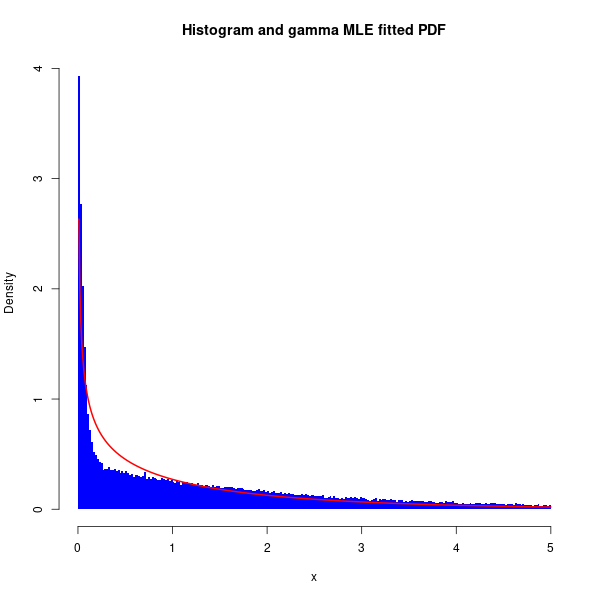
\includegraphics[scale=0.75]{images/Histogram-and-fitted-gamma-PDF}
\end{figure}

Figure 3 displays a histogram of the 100,000 observations as well
as a gamma distribution fitted via Maximum Likelihood Estimation (MLE).
The estimated shape and scale parameters of the gamma distribution
are 0.61 and 2.03, respectively (the exact value are unimportant).
The gamma distribution comes reasonably close to the histogram, but
the match is not great.

An alternative estimator of $g(x)$ is a kernel density estimator.
Figure 4 displays a comparison of the MLE gamma estimate of $g(x)$,
the kernel density estimate, and the true $g(x)$. From this we can
see that the kernel density estimator performs quite well, while the
gamma MLE curve traces out significant gaps.

\begin{figure}
\caption{}

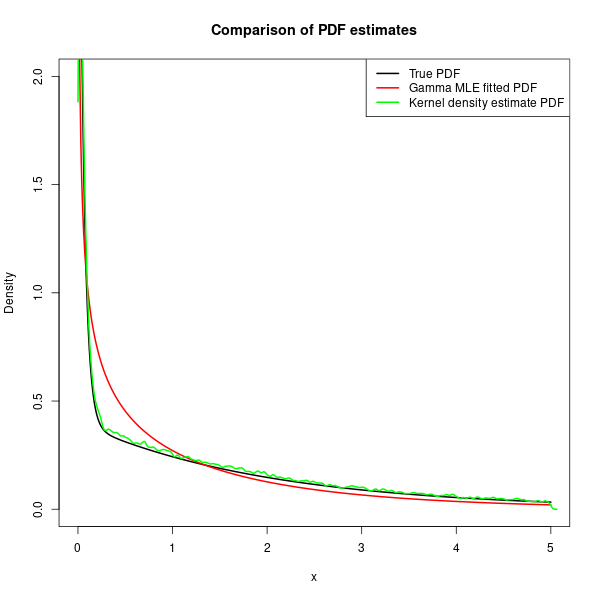
\includegraphics[scale=0.75]{images/Comparison-of-PDF-estimates}
\end{figure}

This can be seen more clearly in a plot of the estimated cumulative
distribution function (CDF) of the gamma MLE and the empirical distribution
of the simulated data drawn from $g(x)$, as in Figure 5. The Kolmogorov--Smirnov
statistic for the difference between these two distributions is 0.0615.
By contrast, the CDFs of the kernel density estimate and the empirical
distribution of the simulated data are difficult to distinguish visually
in Figure 6. The Kolmogorov--Smirnov statistic here is 0.0094, which
is nearly an order-of-magnitude improvement over the MLE gamma estimate.
Note that here kernel density estimation is operating at a disadvantage
since the true distribution is very discontinuous at 0.

\begin{figure}
\caption{}

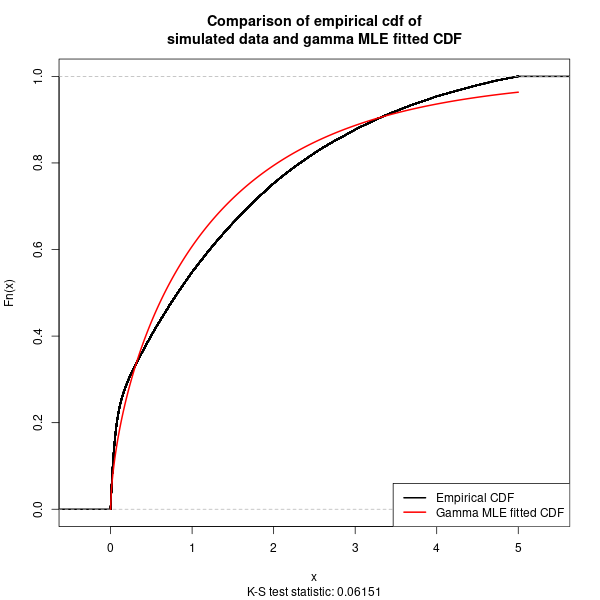
\includegraphics[scale=0.75]{images/Comparison-of-CDF-gamma}
\end{figure}

\begin{figure}
\caption{}

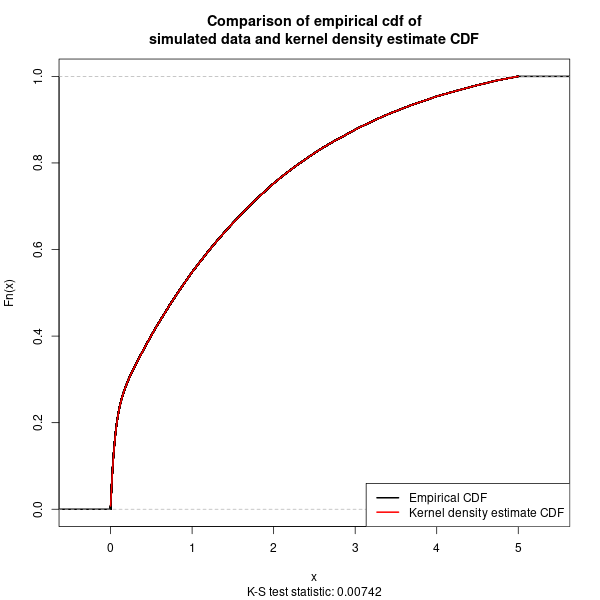
\includegraphics[scale=0.75]{images/Comparison-of-CDF-kernel-density}
\end{figure}


\section{Statistical properties of nonparametric estimators of PDFs}

Let $h$ be the bandwidth of $\hat{f_{S}}(x)$ , a kernel density
estimator of $f_{S}(x)$. Under the assumption that $f_{S}(x)$ is
continuous (an assumption that is approximately correct for the empirical
Monero output spend-age data, except at the zero boundary) with $n$
being the number of observations used in the estimation, it can be
shown that

\begin{equation}
\mathrm{as\:}h\rightarrow0\mathrm{\:and\:}nh\rightarrow\infty,\hat{f_{S}}(x)\overset{p}{\longrightarrow}f_{S}(x)
\end{equation}

i.e. the estimator $\hat{f_{S}}(x)$ converges in probability to the
true distribution $f_{S}(x)$.

Therefore, we have this wonderful result that with a sufficiently
large sample $n$ (and $h$ chosen appropriately), the difference
between $\hat{f_{S}}(x)$ and $f_{S}(x)$ shrinks toward zero. Setting
$f_{M}(x)$ to this nonparametric kernel density estimator $\hat{f_{S}}(x)$
achieves the goal of minimizing the leakage of statistically meaningful
data in a very simple way. We are done! Sort of.

So, why aren't nonparametric methods more widely used in statistical
analysis? I can think of a few reasons:
\begin{enumerate}
\item Your sample size needs to be quite large. As is typical in statistics,
here you do not get something in exchange for nothing. Unsurprisingly,
when you assume more information about your distribution, which is
the case with parametric methods, you need less information from the
empirical sample, so your sample size can be small. Of course, if
you guess wrong, your method falls apart badly, as we have seen. In
technical terms, parametric estimators generally converge at rate
$n^{-1/2}$ while nonparametric estimators converge at a rate slower
than $n^{-1/2}$. With a small sample size, both the bias and variance
terms in nonparametric estimators can be large. Fortunately, the sample
size of Monero transactions is relatively large, so this concern does
not apply.
\item Since you do not obtain a finite set of parameters, nonparametric
methods can inhibit interpretation of results. Many questions in the
natural and social sciences are best answered with a statement about
the estimated value of a specific parameter of a distribution. Non
parametric methods may give you interesting pictures, but their meaning
is often difficult to interpret. This shortcoming of nonparametric
methods does not really apply to the mixin selection algorithm. In
a certain sense we want to thwart any interpretation, in fact.
\item Your research question may not involve the distribution at all, but
just the mean or some other point estimand. This does not apply to
our effort to overhaul the mixin selection algorithm, since applying
the mean is not enough to conceal real spends.
\item The object under study is multivariate. This issue is similar to the
sample size requirements. The complexity of nonparametric methods
increase exponentially, literally, with the number of variables whose
joint PDF you need to estimate. The curse of dimensionality hits nonparametric
methods hard. Since we are only dealing with a univariate probability
distribution, this problem also does not inhibit us from pursuing
nonparametric methods.
\item Non-scientific practical issues. Nonparametric methods are yet another
entire class of statistical methods that need to be learned about.
Researchers just might not be bothered. Peer reviewers may not be
familiar with them. A conference paper may need to be submitted on
a tight deadline and it may be easier to fall back on familiar methods.
None of these issues should concern us; let's reach for the highest
standards of rigor that we can.
\end{enumerate}
Although nonparametric estimation of a univariate probability density
function is relatively basic and well-studied as far as statistical
techniques go, we will face many challenges and choices. Among them
are:
\begin{enumerate}
\item Which type of nonparametric estimator to use. This could be kernel
density, splines, series, or local polynomial density estimators,
and maybe more that I am unaware of.
\item How to determine the tuning parameters. With kernel density estimation,
this is the bandwidth $h$. Other estimators have their corresponding
tuning parameters. There are many different approaches to determining
the value of the tuning parameters, several of them involving cross-validation
techniques. The literature has many suggestions about how to do this,
but none are really \textquotedbl best\textquotedbl{} for all circumstances,
so we will have to investigate many avenues and see how they fit into
our particular problem.
\item How to deal with the fact that $f_{S}(x)$ is literally a moving target.
$f_{S}(x)$ is not static. Presumably, it is evolving through time
as usage patterns change. Therefore, $f_{S}(x)$ is actually a set
of probability distributions indexed by time $t$ as $f_{S,t}(x)$.
\end{enumerate}

\section{OSPEAD: A parametric approach for implementation in the medium term}

The nonparametric approach to the mixin selection algorithm will take
a lot of time to develop and test. In the medium term, it may make
sense to develop a parametric approach that is a large improvement
on the current algorithm, yet is feasible to develop and deploy quickly.
I outline such an approach below.

We have seen that parametric approaches will never be perfect. Inevitably,
they will fail to match the true spend distribution in some ways,
large or small. Due to this unfortunate reality, choosing among various
parametric options directly implies choosing to more strongly protect
the privacy of some users --- and grant less protection to other
users. Or more precisely, the spend-age of some real outputs are better
obfuscated by a greater number of mixins. These tradeoffs cannot be
avoided, and so they must be handled somehow. We may not have asked
to play god with users' privacy, but playing god is inevitable.

Choosing which users to protect ultimately is not a technical question.
It is a normative question. That is to say, it is not a question about
\textit{what is}. \textquotedbl What is\textquotedbl{} can often
be answered with enough research effort by technicians. Normative
questions are concerned with what ought to be. Within a traditional
framework, \textquotedbl society\textquotedbl{} or \textquotedbl policymakers\textquotedbl{}
would answer these questions. Within the Monero context, the groups
answering these questions may be Monero devs, the Monero Research
Lab, and Monero community members who are willing to understand the
issues at hand. Technical researchers can present the answers to positive
questions that help inform the deliberations about the normative questions,
but they alone cannot make the final call on these matters.

The discipline of economics tackles frequently these questions about
trading off one individual's welfare for that of another, so I will
bring in some economic concepts. But first, some mathematical setup.
As before,

Let $f_{S}(x)$ denote the probability density function (PDF) of the
age of the real spend outputs of transactions on the Monero blockchain.

Let $f_{M}(x)$ denote the PDF of the age of the mixins used by the
reference wallet software for Monero. Now define the following function:

$h(x)=\max\left\{ 0,f_{S}(x)-f_{M}(x)\right\} $

At any particular value $x$, then, $h(x)$ is the \textquotedbl privacy
deficit\textquotedbl{} suffered by a user who chooses to spend an
output that has age$x$ . For the current purposes, additional privacy
coverage above the target level of $f_{S}(x)=f_{M}(x)$ will be considered
of no benefit, partly because for any interval on the support of $f_{S}(x)$
and $f_{M}(x)$ for which $f_{S}(x)<f_{M}(x)$ inevitably results
in another interval that will have a privacy deficit, due to the zero-sum
nature of the probability distributions.

How do we construct $f_{M}(x)$ for best overall privacy if we restrict
ourselves to parametric distributions, and therefore cannot achieve
$f_{S}(x)\approx f_{M}(x)$ for all values of $x$? Well, it depend
on how we define \textquotedbl best\textquotedbl . Below are six
approaches. I have the mathematical definitions of these worked out
in my head, but they are not written here:

$\vphantom{}$

1) Privacy impoverishment

2) Economic welfare

3) Inequality minimization

4) Worst-case-scenario minimization

5) Maximum Likelihood Estimation

6) Maximize resistance to a specific attack (likely the RRA) {[}this
item may be redacted before release{]}

$\vphantom{}$

Now that a set of objective functions have been defined, one could
imagine optimizing these objective functions in a numerical optimization
procedure where each parametric distribution family with support of
$[0,\infty)$ is permuted over 1-6 above.

I call this approach Optimal Static Parametric Estimation of Arbitrary
Distributions (OSPEAD), which is an acronym that I just made up so
that it can be referred to by a name in discussions in the Monero
Research Lab and the wider Monero community. It is ``Optimal'' in
some sense, at least in reference to one of the six criteria outlined
above. It is ``Static'' in that it is not dynamic. An estimate is
made once, then implemented and released, and is not adjusted depending
on temporal shifts in $f_{S}(x)$. It is a ``Parametric Estimation''
since it is parametric. The estimation is done of an ``Arbitrary
Distribution'' since the real spend distribution is not a specific
parametric one, but is in some sense ``arbitrary''.\\

\noindent\doublebox{\begin{minipage}[t]{1\columnwidth - 2\fboxsep - 7.5\fboxrule - 1pt}%
\begin{description}
\item [{\textbf{Recommendation}}] \textbf{V}: As a medium-term solution
to ``stop the bleeding'', the Monero Project should work to operationalize
Optimal Static Parametric Estimation of Arbitrary Distributions (OSPEAD).
Implementation of OSPEAD would require to completion of much of the
initial work to estimate $f_{S}(x)$ that would also be required for
the nonparametric approach, so not much extra labor would need to
be expended to implement OSPEAD.
\end{description}
%
\end{minipage}}

\pagebreak{}

\appendix

\section{Appendix: Data for Figure 2: Simulated guessibility as a function
of ring size}

\begin{tabular}{|c|c|}
\hline 
ring.size & guessibility\tabularnewline
\hline 
\hline 
2 & 72.5012\tabularnewline
\hline 
3 & 60.5882\tabularnewline
\hline 
4 & 53.5727\tabularnewline
\hline 
5 & 48.7711\tabularnewline
\hline 
6 & 45.3109\tabularnewline
\hline 
7 & 42.573\tabularnewline
\hline 
8 & 40.331\tabularnewline
\hline 
9 & 38.4334\tabularnewline
\hline 
10 & 36.8847\tabularnewline
\hline 
11 & 35.4512\tabularnewline
\hline 
12 & 34.2561\tabularnewline
\hline 
13 & 33.0742\tabularnewline
\hline 
14 & 32.0973\tabularnewline
\hline 
15 & 31.2342\tabularnewline
\hline 
16 & 30.3308\tabularnewline
\hline 
17 & 29.7038\tabularnewline
\hline 
18 & 28.9702\tabularnewline
\hline 
19 & 28.2215\tabularnewline
\hline 
20 & 27.6658\tabularnewline
\hline 
21 & 27.0826\tabularnewline
\hline 
22 & 26.5358\tabularnewline
\hline 
23 & 26.0151\tabularnewline
\hline 
24 & 25.5879\tabularnewline
\hline 
25 & 25.1412\tabularnewline
\hline 
26 & 24.7264\tabularnewline
\hline 
27 & 24.3091\tabularnewline
\hline 
28 & 23.9704\tabularnewline
\hline 
29 & 23.6244\tabularnewline
\hline 
30 & 23.223\tabularnewline
\hline 
31 & 22.969\tabularnewline
\hline 
32 & 22.5744\tabularnewline
\hline 
33 & 22.3436\tabularnewline
\hline 
34 & 21.9896\tabularnewline
\hline 
35 & 21.726\tabularnewline
\hline 
36 & 21.476\tabularnewline
\hline 
37 & 21.1885\tabularnewline
\hline 
38 & 20.9454\tabularnewline
\hline 
39 & 20.679\tabularnewline
\hline 
40 & 20.4868\tabularnewline
\hline 
\end{tabular}$\;$%
\begin{tabular}{|c|c|}
\hline 
ring.size & guessibility\tabularnewline
\hline 
\hline 
41 & 20.2236\tabularnewline
\hline 
42 & 20.0369\tabularnewline
\hline 
43 & 19.7598\tabularnewline
\hline 
44 & 19.554\tabularnewline
\hline 
45 & 19.4144\tabularnewline
\hline 
46 & 19.1737\tabularnewline
\hline 
47 & 19.009\tabularnewline
\hline 
48 & 18.7778\tabularnewline
\hline 
49 & 18.7009\tabularnewline
\hline 
50 & 18.4791\tabularnewline
\hline 
51 & 18.2825\tabularnewline
\hline 
52 & 18.1669\tabularnewline
\hline 
53 & 18.0036\tabularnewline
\hline 
54 & 17.8241\tabularnewline
\hline 
55 & 17.7633\tabularnewline
\hline 
56 & 17.4893\tabularnewline
\hline 
57 & 17.3701\tabularnewline
\hline 
58 & 17.2866\tabularnewline
\hline 
59 & 17.1557\tabularnewline
\hline 
60 & 17.057\tabularnewline
\hline 
61 & 16.8666\tabularnewline
\hline 
62 & 16.7201\tabularnewline
\hline 
63 & 16.6219\tabularnewline
\hline 
64 & 16.5125\tabularnewline
\hline 
65 & 16.3744\tabularnewline
\hline 
66 & 16.2666\tabularnewline
\hline 
67 & 16.0869\tabularnewline
\hline 
68 & 16.0288\tabularnewline
\hline 
69 & 15.9613\tabularnewline
\hline 
70 & 15.7724\tabularnewline
\hline 
71 & 15.6817\tabularnewline
\hline 
72 & 15.5569\tabularnewline
\hline 
73 & 15.5948\tabularnewline
\hline 
74 & 15.4265\tabularnewline
\hline 
75 & 15.2845\tabularnewline
\hline 
76 & 15.1892\tabularnewline
\hline 
77 & 15.0941\tabularnewline
\hline 
78 & 15.0289\tabularnewline
\hline 
79 & 14.9434\tabularnewline
\hline 
\end{tabular}$\;$%
\begin{tabular}{|c|c|}
\hline 
ring.size & guessibility\tabularnewline
\hline 
\hline 
80 & 14.8169\tabularnewline
\hline 
81 & 14.7812\tabularnewline
\hline 
82 & 14.7143\tabularnewline
\hline 
83 & 14.6116\tabularnewline
\hline 
84 & 14.5225\tabularnewline
\hline 
85 & 14.4465\tabularnewline
\hline 
86 & 14.3477\tabularnewline
\hline 
87 & 14.2993\tabularnewline
\hline 
88 & 14.1777\tabularnewline
\hline 
89 & 14.1945\tabularnewline
\hline 
90 & 14.0879\tabularnewline
\hline 
91 & 13.9317\tabularnewline
\hline 
92 & 13.9423\tabularnewline
\hline 
93 & 13.8525\tabularnewline
\hline 
94 & 13.6843\tabularnewline
\hline 
95 & 13.7098\tabularnewline
\hline 
96 & 13.5968\tabularnewline
\hline 
97 & 13.5883\tabularnewline
\hline 
98 & 13.5198\tabularnewline
\hline 
99 & 13.4686\tabularnewline
\hline 
100 & 13.3782\tabularnewline
\hline 
101 & 13.3063\tabularnewline
\hline 
102 & 13.2141\tabularnewline
\hline 
103 & 13.1253\tabularnewline
\hline 
104 & 13.1035\tabularnewline
\hline 
105 & 13.1477\tabularnewline
\hline 
106 & 12.9838\tabularnewline
\hline 
107 & 12.9447\tabularnewline
\hline 
108 & 12.8793\tabularnewline
\hline 
109 & 12.8533\tabularnewline
\hline 
110 & 12.7135\tabularnewline
\hline 
111 & 12.7847\tabularnewline
\hline 
112 & 12.678\tabularnewline
\hline 
113 & 12.5874\tabularnewline
\hline 
114 & 12.5281\tabularnewline
\hline 
115 & 12.5641\tabularnewline
\hline 
116 & 12.4443\tabularnewline
\hline 
117 & 12.4087\tabularnewline
\hline 
118 & 12.3086\tabularnewline
\hline 
\end{tabular}$\;$%
\begin{tabular}{|c|c|}
\hline 
ring.size & guessibility\tabularnewline
\hline 
\hline 
119 & 12.3242\tabularnewline
\hline 
120 & 12.2153\tabularnewline
\hline 
121 & 12.2247\tabularnewline
\hline 
122 & 12.1439\tabularnewline
\hline 
123 & 12.02\tabularnewline
\hline 
124 & 12.0437\tabularnewline
\hline 
125 & 11.9673\tabularnewline
\hline 
126 & 11.9857\tabularnewline
\hline 
127 & 11.9378\tabularnewline
\hline 
128 & 11.9138\tabularnewline
\hline 
129 & 11.8292\tabularnewline
\hline 
130 & 11.7355\tabularnewline
\hline 
131 & 11.6984\tabularnewline
\hline 
132 & 11.6925\tabularnewline
\hline 
133 & 11.5679\tabularnewline
\hline 
134 & 11.6183\tabularnewline
\hline 
135 & 11.611\tabularnewline
\hline 
136 & 11.5642\tabularnewline
\hline 
137 & 11.4979\tabularnewline
\hline 
138 & 11.4401\tabularnewline
\hline 
139 & 11.3759\tabularnewline
\hline 
140 & 11.3705\tabularnewline
\hline 
141 & 11.3613\tabularnewline
\hline 
142 & 11.3329\tabularnewline
\hline 
143 & 11.2314\tabularnewline
\hline 
144 & 11.2338\tabularnewline
\hline 
145 & 11.2552\tabularnewline
\hline 
146 & 11.112\tabularnewline
\hline 
147 & 11.1354\tabularnewline
\hline 
148 & 11.0326\tabularnewline
\hline 
149 & 11.0269\tabularnewline
\hline 
150 & 10.9913\tabularnewline
\hline 
151 & 10.9753\tabularnewline
\hline 
152 & 10.9195\tabularnewline
\hline 
153 & 10.8727\tabularnewline
\hline 
154 & 10.869\tabularnewline
\hline 
155 & 10.8385\tabularnewline
\hline 
156 & 10.8104\tabularnewline
\hline 
157 & 10.7796\tabularnewline
\hline 
\end{tabular}\\
\begin{tabular}{|c|c|}
\hline 
ring.size & guessibility\tabularnewline
\hline 
\hline 
158 & 10.7091\tabularnewline
\hline 
159 & 10.737\tabularnewline
\hline 
160 & 10.6777\tabularnewline
\hline 
161 & 10.5986\tabularnewline
\hline 
162 & 10.5744\tabularnewline
\hline 
163 & 10.5658\tabularnewline
\hline 
164 & 10.6061\tabularnewline
\hline 
165 & 10.5429\tabularnewline
\hline 
166 & 10.4849\tabularnewline
\hline 
167 & 10.4605\tabularnewline
\hline 
168 & 10.4554\tabularnewline
\hline 
169 & 10.3781\tabularnewline
\hline 
170 & 10.3693\tabularnewline
\hline 
171 & 10.4257\tabularnewline
\hline 
172 & 10.278\tabularnewline
\hline 
173 & 10.2189\tabularnewline
\hline 
174 & 10.2221\tabularnewline
\hline 
175 & 10.2294\tabularnewline
\hline 
176 & 10.1971\tabularnewline
\hline 
177 & 10.1301\tabularnewline
\hline 
178 & 10.1307\tabularnewline
\hline 
179 & 10.1001\tabularnewline
\hline 
180 & 10.0472\tabularnewline
\hline 
181 & 10.0499\tabularnewline
\hline 
182 & 10.0953\tabularnewline
\hline 
183 & 9.9882\tabularnewline
\hline 
184 & 10.0144\tabularnewline
\hline 
185 & 9.9966\tabularnewline
\hline 
186 & 9.9496\tabularnewline
\hline 
187 & 9.8963\tabularnewline
\hline 
188 & 9.9196\tabularnewline
\hline 
189 & 9.8669\tabularnewline
\hline 
190 & 9.8523\tabularnewline
\hline 
191 & 9.8212\tabularnewline
\hline 
192 & 9.8059\tabularnewline
\hline 
193 & 9.7326\tabularnewline
\hline 
194 & 9.7259\tabularnewline
\hline 
195 & 9.7009\tabularnewline
\hline 
196 & 9.6776\tabularnewline
\hline 
\end{tabular}$\;$%
\begin{tabular}{|c|c|}
\hline 
ring.size & guessibility\tabularnewline
\hline 
\hline 
197 & 9.6471\tabularnewline
\hline 
198 & 9.6864\tabularnewline
\hline 
199 & 9.6766\tabularnewline
\hline 
200 & 9.6163\tabularnewline
\hline 
201 & 9.6361\tabularnewline
\hline 
202 & 9.5289\tabularnewline
\hline 
203 & 9.6106\tabularnewline
\hline 
204 & 9.5042\tabularnewline
\hline 
205 & 9.5099\tabularnewline
\hline 
206 & 9.47\tabularnewline
\hline 
207 & 9.4584\tabularnewline
\hline 
208 & 9.4641\tabularnewline
\hline 
209 & 9.4164\tabularnewline
\hline 
210 & 9.3728\tabularnewline
\hline 
211 & 9.4003\tabularnewline
\hline 
212 & 9.2914\tabularnewline
\hline 
213 & 9.2962\tabularnewline
\hline 
214 & 9.3481\tabularnewline
\hline 
215 & 9.3238\tabularnewline
\hline 
216 & 9.1997\tabularnewline
\hline 
217 & 9.2272\tabularnewline
\hline 
218 & 9.2353\tabularnewline
\hline 
219 & 9.1923\tabularnewline
\hline 
220 & 9.2664\tabularnewline
\hline 
221 & 9.182\tabularnewline
\hline 
222 & 9.1696\tabularnewline
\hline 
223 & 9.1212\tabularnewline
\hline 
224 & 9.0993\tabularnewline
\hline 
225 & 9.0391\tabularnewline
\hline 
226 & 9.0986\tabularnewline
\hline 
227 & 9.0873\tabularnewline
\hline 
228 & 9.0834\tabularnewline
\hline 
229 & 9.0083\tabularnewline
\hline 
230 & 9.0087\tabularnewline
\hline 
231 & 9.0171\tabularnewline
\hline 
232 & 9.0024\tabularnewline
\hline 
233 & 8.9709\tabularnewline
\hline 
234 & 8.9839\tabularnewline
\hline 
235 & 8.8782\tabularnewline
\hline 
\end{tabular}$\;$%
\begin{tabular}{|c|c|}
\hline 
ring.size & guessibility\tabularnewline
\hline 
\hline 
236 & 8.8911\tabularnewline
\hline 
237 & 8.8736\tabularnewline
\hline 
238 & 8.8214\tabularnewline
\hline 
239 & 8.8351\tabularnewline
\hline 
240 & 8.8778\tabularnewline
\hline 
241 & 8.8049\tabularnewline
\hline 
242 & 8.8286\tabularnewline
\hline 
243 & 8.7642\tabularnewline
\hline 
244 & 8.7327\tabularnewline
\hline 
245 & 8.7567\tabularnewline
\hline 
246 & 8.6941\tabularnewline
\hline 
247 & 8.7275\tabularnewline
\hline 
248 & 8.6634\tabularnewline
\hline 
249 & 8.6805\tabularnewline
\hline 
250 & 8.69\tabularnewline
\hline 
251 & 8.6107\tabularnewline
\hline 
252 & 8.5447\tabularnewline
\hline 
253 & 8.6345\tabularnewline
\hline 
254 & 8.5343\tabularnewline
\hline 
255 & 8.5823\tabularnewline
\hline 
256 & 8.5382\tabularnewline
\hline 
 & \tabularnewline
\hline 
 & \tabularnewline
\hline 
 & \tabularnewline
\hline 
 & \tabularnewline
\hline 
 & \tabularnewline
\hline 
 & \tabularnewline
\hline 
 & \tabularnewline
\hline 
 & \tabularnewline
\hline 
 & \tabularnewline
\hline 
 & \tabularnewline
\hline 
 & \tabularnewline
\hline 
 & \tabularnewline
\hline 
 & \tabularnewline
\hline 
 & \tabularnewline
\hline 
 & \tabularnewline
\hline 
 & \tabularnewline
\hline 
 & \tabularnewline
\hline 
 & \tabularnewline
\hline 
\end{tabular}

\section{Appendix: Rucknium Ratio Attack Monte Carlo R Code}

\noindent\fbox{\begin{minipage}[t]{1\columnwidth - 2\fboxsep - 2\fboxrule}%
\texttt{xmr <- read.csv(\textquotedbl output\_age\_data.csv\textquotedbl ,
stringsAsFactors = FALSE)}

\texttt{\# From https://github.com/monero-project/monero/files/6968268/output\_age\_data.zip}

\texttt{xmr\$Observed.pdf <- xmr\$Observed/sum(xmr\$Observed)}

\texttt{\# Convert f(x) to a \textquotedbl probability density function\textquotedbl ,
more or less}

\texttt{xmr\$Current.decoy.selection.algo.pdf <- xmr\$Current.decoy.selection.algo
/ }

\texttt{sum(xmr\$Current.decoy.selection.algo)}

\texttt{\# Do the same for f\_M(x)}

\texttt{alpha <- 10/11}

\texttt{xmr\$f\_S <- (1/(1-alpha)) {*} }

\texttt{(xmr\$Observed.pdf - alpha {*} xmr\$Current.decoy.selection.algo.pdf)}

\texttt{\# Construct f\_S(x) according to equation (2) in the paper}

\texttt{xmr\$f\_S{[}xmr\$f\_S < 0{]} <- xmr\$Current.decoy.selection.algo.pdf{[}xmr\$f\_S
< 0{]}}

\texttt{\# Sometimes the observed can be below what the idealized
algorithm would have }

\texttt{\# selected since there is noise in the long tails. }

\texttt{xmr\$f\_S <- xmr\$f\_S / sum(xmr\$f\_S)}

\texttt{\# Make f\_S(x) be a proper PDF}

\texttt{xmr\$Rucknium.Ratio <- xmr\$f\_S / xmr\$Current.decoy.selection.algo.pdf}

\texttt{png(\textquotedbl Rucknium-Ratio.png\textquotedbl , width
= 600, height = 600)}

\texttt{par(mar = c(5, 6, 4, 2) + 0.1)}

\texttt{\# c(5, 4, 4, 2) + 0.1}

\texttt{plot(xmr\$Rucknium.Ratio{[}1:10000{]}, log = \textquotedbl x\textquotedbl ,
cex = 0.5, }

\texttt{col = rgb(0, 0, 0, alpha = c(rep(1, 100), rep(0, 9900))),}

\texttt{main = \textquotedbl Rucknium Ratio\textbackslash nDots
are partially transparent for better visualization\textquotedbl ,}

\texttt{xlab = \textquotedbl Age of blocks corresponding to ring
members (log scale)\textquotedbl ,}

\texttt{ylab = expression(\textquotedbl Rucknium Ratio \textquotedbl{}
{*} frac(f{[}S{]}(x), f{[}M{]}(x))) )}

\texttt{lines(x = 1:100, y = xmr\$Rucknium.Ratio{[}1:100{]})}

\texttt{points(x = 101:10000, y = xmr\$Rucknium.Ratio{[}101:10000{]},
col = rgb(0, 0, 0, alpha = 0.2), pch = \textquotedbl .\textquotedbl )}

\texttt{abline(h = 1, lty = 2, col = \textquotedbl red\textquotedbl )}

\texttt{axis(2, 1, \textquotedbl 1\textquotedbl )}

\texttt{dev.off()}

\texttt{par(mar = c(5, 4, 4, 2) + 0.1 )}

\texttt{sum(xmr{[}1:10, \textquotedbl f\_S\textquotedbl{]})}

\texttt{\# {[}1{]} 0.1380584}

\texttt{sum(xmr{[}1:10, \textquotedbl Current.decoy.selection.algo.pdf\textquotedbl{]})}

\texttt{\# {[}1{]} 0.02727423}

\texttt{sum(xmr{[}1:3, \textquotedbl f\_S\textquotedbl{]})}

\texttt{\# {[}1{]} 0.05523403}

\texttt{sum(xmr{[}1:3, \textquotedbl Current.decoy.selection.algo.pdf\textquotedbl{]})}

\texttt{\# {[}1{]} 0.005761155}

\texttt{set.seed(314)}

\texttt{n.rings <- 10000000}

\texttt{\# 10 million}%
\end{minipage}}

\noindent\fbox{\begin{minipage}[t]{1\columnwidth - 2\fboxsep - 2\fboxrule}%
\texttt{simulation.mixin.quantity <- 10}

\texttt{rings <- matrix(c(}

\texttt{sample(nrow(xmr), size = simulation.mixin.quantity {*} n.rings,
replace = TRUE, }

\texttt{prob = xmr\$Current.decoy.selection.algo.pdf),}

\texttt{sample(nrow(xmr), size = 1 {*} n.rings, replace = TRUE, prob
= xmr\$f\_S)}

\texttt{), byrow = FALSE, ncol = simulation.mixin.quantity + 1)}

\texttt{attack.prob.11 <- apply(rings, 1, FUN = function(x) \{}

\texttt{which.max(xmr\$Rucknium.Ratio{[}x{]})}

\texttt{\})}

\texttt{\# Note that which.max() returns the index of the \textquotedbl first\textquotedbl{}
maximum if the maximum}

\texttt{\# is not unique. Therefore, the real spend was chosen to
be the \textquotedbl last\textquotedbl}

\texttt{\# element of the set so that it would be clear that the real
spend, if}

\texttt{\# guessed, was the result of unique guess}

\texttt{t(t(100 {*} prop.table(table(attack.prob.11)) ))}

\texttt{\# Main result}

\texttt{\#\#\#\#\#\#\#\#\#\#\#\#\#\#\#\#\#\#\#\#\#\#\#\#\#\#\#\#\#\#\#\#\#\#\#\#\#\#\#\#\#\#\#\#\#\#\#\#\#\#\#\#\#\#\#\#\#\#\#\#\#\#}

\texttt{\# Simulation for different ring sizes follows}

\texttt{\# Note: This takes about an hour to run}

\texttt{\#\#\#\#\#\#\#\#\#\#\#\#\#\#\#\#\#\#\#\#\#\#\#\#\#\#\#\#\#\#\#\#\#\#\#\#\#\#\#\#\#\#\#\#\#\#\#\#\#\#\#\#\#\#\#\#\#\#\#\#\#\#}

\texttt{set.seed(314)}

\texttt{n.rings <- 1000000}

\texttt{\# 1 million}

\texttt{max.ring.size <- 256}

\texttt{guessibility.results <- list()}

\texttt{for (i in seq\_len(max.ring.size - 1)) \{}

\texttt{simulation.mixin.quantity <- i}

\texttt{rings <- matrix(c(}

\texttt{sample(nrow(xmr), size = simulation.mixin.quantity {*} n.rings,
replace = TRUE, prob = xmr\$Current.decoy.selection.algo.pdf),}

\texttt{sample(nrow(xmr), size = 1 {*} n.rings, replace = TRUE, prob
= xmr\$f\_S)}

\texttt{), byrow = FALSE, ncol = simulation.mixin.quantity + 1)}

\texttt{xmr\$Rucknium.Ratio <- xmr\$f\_S / xmr\$Current.decoy.selection.algo.pdf}

\texttt{attack.prob <- apply(rings, 1, FUN = function(x) \{}

\texttt{which.max(xmr\$Rucknium.Ratio{[}x{]})}

\texttt{\})}

\texttt{guessibility.results{[}{[}i{]}{]} <- t(t(100 {*} prop.table(table(attack.prob))
))}

\texttt{print( guessibility.results{[}{[}i{]}{]})}

\texttt{\}}

\texttt{guessibility <- sapply( guessibility.results, FUN = function(x)
\{}

\texttt{x{[}nrow(x), {]}}

\texttt{\})}

\texttt{guessibility <- unname(guessibility)}%
\end{minipage}}

\noindent\fbox{\begin{minipage}[t]{1\columnwidth - 2\fboxsep - 2\fboxrule}%
\texttt{png(\textquotedbl Guessibility-by-ring-size.png\textquotedbl ,
width = 600, height = 600)}

\texttt{plot(seq\_along(guessibility) + 1, guessibility, ylim = c(0,
max(guessibility)), }

\texttt{cex = 0.25, }

\texttt{main = \textquotedbl Simulated guessibility as a function
of ring size\textquotedbl ,}

\texttt{xlab = \textquotedbl Ring size\textquotedbl ,}

\texttt{ylab = \textquotedbl Pr(guess real spend correctly | R)\textquotedbl )}

\texttt{abline(v = 11, lty = 2, col = \textquotedbl red\textquotedbl )}

\texttt{axis(1, 11, \textquotedbl 11\textquotedbl )}

\texttt{dev.off()}

\texttt{guessibility.data.frame <- data.frame(ring.size = seq\_along(guessibility)
+ 1, guessibility = guessibility)}

\texttt{summary(lm(log(guessibility) \textasciitilde{} ring.size,
data = guessibility.data.frame))}

\texttt{write.csv(guessibility.data.frame, }

\texttt{file = \textquotedbl Guessibility-by-ring-size-data.csv\textquotedbl ,
row.names = FALSE)}%
\end{minipage}}

\pagebreak{}

\section{Appendix: Comparison of Maximum Likelihood Estimation and Nonparametric
Estimation of Simulated Mixture Distribution}

\noindent\fbox{\begin{minipage}[t]{1\columnwidth - 2\fboxsep - 2\fboxrule}%
\texttt{\# install.packages(\textquotedbl distr\textquotedbl )}

\texttt{\# install.packages(\textquotedbl fitdistrplus\textquotedbl )}

\texttt{\# install.packages(\textquotedbl ks\textquotedbl )}

\texttt{\# library(ks)}

\texttt{\# library(distr)}

\texttt{\# library(fitdistrplus)}

\texttt{set.seed(314)}

\texttt{n.obs <- 100000}

\texttt{x.trunc <- 5}

\texttt{mixed.dist <- distr::UnivarMixingDistribution(}

\texttt{distr::Exp(20), }

\texttt{distr::Chisq(df = 2),}

\texttt{mixCoeff = c(0.2, 0.8))}

\texttt{r.mixed.dist <- distr::r(mixed.dist)}

\texttt{d.mixed.dist <- distr::d(mixed.dist)}

\texttt{x <- r.mixed.dist(n.obs)}

\texttt{x <- x{[}x <= x.trunc{]}}

\texttt{length(x)}

\texttt{summary(x)}

\texttt{hist(x, breaks = 200, freq = FALSE, col = \textquotedbl blue\textquotedbl ,
border = NA)}

\texttt{mle.gamma <- fitdistrplus::fitdist(x, \textquotedbl gamma\textquotedbl ,
start = list(shape = 2, scale = 2))}

\texttt{png(\textquotedbl Histogram-and-fitted-gamma-PDF.png\textquotedbl ,
width = 600, height = 600)}

\texttt{hist(x, breaks = 200, freq = FALSE, col = \textquotedbl blue\textquotedbl ,
border = NA,}

\texttt{main = \textquotedbl Histogram and gamma MLE fitted PDF\textquotedbl )}

\texttt{lines(}

\texttt{seq(0, x.trunc, by = 0.01),}

\texttt{dgamma(seq(0, x.trunc, by = 0.01), shape = mle.gamma\$estimate{[}\textquotedbl shape\textquotedbl{]},
scale = mle.gamma\$estimate{[}\textquotedbl scale\textquotedbl{]}), }

\texttt{col = \textquotedbl red\textquotedbl , lwd = 2)}

\texttt{dev.off()}

\texttt{kde.est <- ks::kde(x, gridsize = 5000) }

\texttt{x.seq <- seq(0, x.trunc, length.out = 500)}%
\end{minipage}}

\noindent\fbox{\begin{minipage}[t]{1\columnwidth - 2\fboxsep - 2\fboxrule}%
\texttt{png(\textquotedbl Comparison-of-PDF-estimates.png\textquotedbl ,
width = 600, height = 600)}

\texttt{plot(0, 0, xlim = c(0, x.trunc), }

\texttt{ylim = c(0, 2),}

\texttt{col = \textquotedbl transparent\textquotedbl ,}

\texttt{xlab = \textquotedbl x\textquotedbl ,}

\texttt{ylab = \textquotedbl Density\textquotedbl ,}

\texttt{main = \textquotedbl Comparison of PDF estimates\textquotedbl )}

\texttt{legend( \textquotedbl topright\textquotedbl ,}

\texttt{legend = c(\textquotedbl True PDF\textquotedbl , \textquotedbl Gamma
MLE fitted PDF\textquotedbl , \textquotedbl Kernel density estimate
PDF\textquotedbl ),}

\texttt{col = c(\textquotedbl black\textquotedbl , \textquotedbl red\textquotedbl ,
\textquotedbl green\textquotedbl ),}

\texttt{lty = 1, lwd = 2)}

\texttt{lines(x.seq, d.mixed.dist(x.seq), col = \textquotedbl black\textquotedbl ,
lwd = 2)}

\texttt{lines(x.seq,}

\texttt{dgamma(x.seq, shape = mle.gamma\$estimate{[}\textquotedbl shape\textquotedbl{]},
scale = mle.gamma\$estimate{[}\textquotedbl scale\textquotedbl{]}), }

\texttt{col = \textquotedbl red\textquotedbl , lwd = 2)}

\texttt{lines(kde.est\$eval.points{[}kde.est\$eval.points > 0{]}, }

\texttt{kde.est\$estimate{[}kde.est\$eval.points > 0{]}, col = \textquotedbl green\textquotedbl ,
lwd = 2)}

\texttt{dev.off()}

\texttt{ks.test.gamma<- ks.test(x, pgamma, shape = mle.gamma\$estimate{[}\textquotedbl shape\textquotedbl{]},
scale = mle.gamma\$estimate{[}\textquotedbl scale\textquotedbl{]})}

\texttt{ks.test.gamma}

\texttt{png(\textquotedbl Comparison-of-CDF-gamma.png\textquotedbl ,
width = 600, height = 600)}

\texttt{plot(ecdf(x), do.points = FALSE, col = \textquotedbl black\textquotedbl ,
lwd = 2, }

\texttt{main = \textquotedbl Comparison of empirical cdf of\textbackslash nsimulated
data and gamma MLE fitted CDF\textquotedbl ,}

\texttt{sub = paste0(\textquotedbl K-S test statistic: \textquotedbl ,
round(ks.test.gamma\$statistic, digits = 5))) }

\texttt{lines(seq(0, x.trunc, by = 0.01), col = \textquotedbl red\textquotedbl ,
lwd = 2,}

\texttt{pgamma(seq(0, x.trunc, by = 0.01), shape = mle.gamma\$estimate{[}\textquotedbl shape\textquotedbl{]},
scale = mle.gamma\$estimate{[}\textquotedbl scale\textquotedbl{]}))}

\texttt{legend( \textquotedbl bottomright\textquotedbl ,}

\texttt{legend = c(\textquotedbl Empirical CDF\textquotedbl , \textquotedbl Gamma
MLE fitted CDF\textquotedbl ),}

\texttt{col = c(\textquotedbl black\textquotedbl , \textquotedbl red\textquotedbl ),}

\texttt{lty = 1, lwd = 2)}

\texttt{dev.off()}

\texttt{kde.cdf.est <- ks::kcde(x, gridsize = 5000)}

\texttt{kde.cdf.est.fun <- approxfun(kde.cdf.est\$eval.points, kde.cdf.est\$estimate,
yleft = 0, yright = 0)}

\texttt{ks.test.kde <- ks.test(x, kde.cdf.est.fun)}

\texttt{ks.test.kde}%
\end{minipage}}

\noindent\fbox{\begin{minipage}[t]{1\columnwidth - 2\fboxsep - 2\fboxrule}%
\texttt{png(\textquotedbl Comparison-of-CDF-kernel-density.png\textquotedbl ,
width = 600, height = 600)}

\texttt{plot(ecdf(x), do.points = FALSE, col = \textquotedbl black\textquotedbl ,
lwd = 2, }

\texttt{main = \textquotedbl Comparison of empirical cdf of\textbackslash nsimulated
data and kernel density estimate CDF\textquotedbl ,}

\texttt{sub = paste0(\textquotedbl K-S test statistic: \textquotedbl ,
round(ks.test.kde\$statistic, digits = 5))) }

\texttt{lines(seq(0, x.trunc, by = 0.01),}

\texttt{kde.cdf.est.fun(seq(0, x.trunc, by = 0.01)), col = \textquotedbl red\textquotedbl ,
lwd = 2) }

\texttt{legend( \textquotedbl bottomright\textquotedbl ,}

\texttt{legend = c(\textquotedbl Empirical CDF\textquotedbl , \textquotedbl Kernel
density estimate CDF\textquotedbl ),}

\texttt{col = c(\textquotedbl black\textquotedbl , \textquotedbl red\textquotedbl ),}

\texttt{lty = 1, lwd = 2)}

\texttt{dev.off()}%
\end{minipage}}
\end{document}
